\documentclass[11pt]{article}

\usepackage[margin=1in]{geometry}
\usepackage{amsmath, amssymb}
\usepackage{graphicx}
\usepackage{float}

\title{Monte Carlo Simulation and Analysis of Gacha Systems}
\author{Alex Hoang\\
\small CECS 381 Stochastic Computing Final Project, Spring 2026}
\date{May 10, 2026}

\begin{document}
\maketitle

% =====================================================================
\section{Problem Description and Motivation}
% =====================================================================

Gacha games are a genre of video games where players can spend in-game currency
on randomized "pulls" to obtain characters and equipment. Two notable examples
are Wuthering Waves and Genshin Impact. Typically, there are two types
of banners: a featured character banner and a featured weapon banner. Each banner has its own
"pity" system, which increases the chances of getting a 5-star item as you pull more times
without success.
This project builds a model of a gacha banner system loosely
based on Wuthering Waves and Genshin Impact, and uses Monte Carlo
simulation to analyze two questions:

\begin{enumerate}
\item How does the simulation compare with an analytical analysis of the gacha system?
\item How does shifting the "soft-pity" onset change the
distribution of pulls a player needs to obtain a full kit from a featured banner set
(a character and a weapon banner)?
\end{enumerate}

% =====================================================================
\section{Model Setup}
% =====================================================================

A gacha system typically has two independent banners: a character banner and a
weapon banner. Pity counters don't transfer between them, so pulling
on one banner doesn't affect the other. They are independent. Table 1 will list 
the variables that are relevant.

\begin{table}[H]
\centering
\caption{Relevant Variables}
\begin{tabular}{lcc}
\hline
Value Type & Symbol & Value \\
\hline
Base 5-star rate (both banners)     & $p_0$       & $0.008$            \\
Hard pity threshold (both)          & $n_h$       & $80$ pulls         \\
Soft-pity onset, character (swept)  & $n_s^c$     & $\{50, 60, 70\}$   \\
Soft-pity onset, weapon (fixed)     & $n_s^w$     & $65$               \\
50/50 win probability, character    & $q$         & $0.5$              \\
Featured rate, weapon               &             & $1.0$              \\
\hline
\end{tabular}
\end{table}

\paragraph{Soft pity ramp.} This mechanic applies to each banner independently.
When used, we will plug in that banner's respective $n_s$ from
Table 1. We will use $n$ to be the number of pulls since the last 5-star. The
per-pull 5-star chance is $p_0$ for the first $n_s - 1$ pulls. Once we hit the soft-pity onset, the probability
begins to ramp up linearly until it hits 1 (which is 100\% probability) at pull $n_h$. 
We can write this as a piecewise function:
\begin{equation}
p_n = \begin{cases}
p_0 & 1 \le n < n_s \\[4pt]
p_0 + \dfrac{n - n_s}{n_h - n_s}(1 - p_0) & n_s \le n \le n_h.
\end{cases}
\end{equation}

In other words, when we hit $n_h$, we will always have a 5-star pull with no
exceptions.

\paragraph{Character-banner 50/50 system.} It should be noted that getting a 5-star on
the character banner doesn't mean that you will get the featured
character. There's a 50/50 chance it's actually some other standard 5-star
character instead. Most gacha games include a guarantee system to ensure that players
can get what they want even if they are unlucky. If you lose the 50/50, then
the next 5-star on that banner is guaranteed to be the featured one. We can actually
look at this like a two-state Markov chain between $\{\text{Fifty-Fifty}, \text{Guarantee}\}$.

\begin{itemize}
 \item In \textbf{Fifty-Fifty}: the player has a 50-50 chance of getting the featured character or 
a standard 5-star character in this state. Thus, the probability $q = 0.5$.
If the player rolls the featured character, they stay in Fifty-Fifty. If not, they move to the Guarantee state.
\item In \textbf{Guarantee}: the next 5-star will be the featured character upon a successful
5-star roll. Upon acquisition, the player moves back to Fifty-Fifty.
\end{itemize}

It should be noted that this system only applies to the character banner.
The weapon banner uses the same soft-pity ramp from
equation (1) with its own onset $n_s^w$. However, it has no fifty-fifty
system: every 5-star on the weapon banner is the featured
weapon.

\paragraph{Full-kit problem.} The player will start with no 5-star
acquisitions, whether it is the character or the weapon. The player will
pull the on the character banner first until they get the featured character. Then
they will switch to the weapon banner until they get the featured weapon. We will track
the number of pulls using variable T.

% =====================================================================
\section{Simulation Methodology}
% =====================================================================

Each pull uses one Uniform(0, 1) draw against the soft-pity
ramp from equation (1) to decide whether it's a 5-star. If we are in the Fifty-Fifty state,
there will be a another draw to determine if we get a standard or featured character. Effectively,
the second draw is a Bernoulli trial. We will run $N = 10^5$ trials of the full kit
problem. The number of trials was chosen as to give us a large enough sample size
to get a good estimation for the expected values.

\paragraph{Analytical reference.} For a given banner, let $N$ be the number of pulls 
until the first 5-star. The probability that this happens on exactly pull $n$ is the chance of
failing the first $n - 1$ pulls and then succeeding on the $n$-th. 
Since the pulls are independent, this is just a product:
\[
P(N = n) = (1 - p_1)(1 - p_2) ... (1 - p_{n-1})(p_n).
\]
An easier way to look at this would be to use product notation. From there, we can plug the
new equation into $\mathbb{E}[X] = \sum x \,P(X=x)$ where X is N:
\begin{equation}
P(N = n) = p_n \prod_{i=1}^{n-1}(1 - p_i),
\qquad
\mathbb{E}[N] = \sum_{n=1}^{n_h} n \,P(N = n).
\end{equation}
We actually can and will compute this using python loops to get an analytical estimation.
From there, we can use it as a reference to check the simulator. For now, we will use
$N_c$ to represent the result of applying these equations to the character banner.

Due to the Fifty-Fifty mechanic, we will use Y to represent the number of pulls to get the
featured character specifically. There are also something else to consider: the player's starting
state. If we start in the Guarantee state, the next 5-star is always featured, so
$\mathbb{E}[Y \mid \text{Guarantee}] = \mathbb{E}[N_c]$. 
If we start in Fifty-Fifty, we have to consider the total expectation of rolling.

This means that there are two scenarios:

\begin{itemize}
\item With probability $q$, we may win the 50/50 on our first 5-star which
takes $\mathbb{E}[N_c]$ pulls on average.
\item With probability $1 - q$ (which should be the same), we may lose the 50/50. 
This moves us to the Guarantee state, and need a second, independent cycle to get 
the guaranteed 5-star. This means that the expected number of pulls should be
$2\,\mathbb{E}[N_c]$. Do note that the first and second cycles are independent.
\end{itemize}

By the law of total expectation, conditioning on whether we win or lose the
first 50/50, the overall expected number of pulls is the weighted sum of the
two conditional expectations:
\[
\mathbb{E}[Y \mid \text{Fifty-Fifty}]
= P(\text{win}) \cdot \mathbb{E}[Y \mid \text{win}]
+ P(\text{lose}) \cdot \mathbb{E}[Y \mid \text{lose}].
\]
Substituting $P(\text{win}) = q$, $P(\text{lose}) = 1 - q$, and the
conditional expectations from the two bullets above:
\begin{equation}
 \mathbb{E}[Y \mid \text{Fifty-Fifty}]
= q\,\mathbb{E}[N_c] + (1 - q)\bigl(2\,\mathbb{E}[N_c]\bigr)
= (2 - q)\,\mathbb{E}[N_c]
= \tfrac{3}{2}\,\mathbb{E}[N_c]
\quad \text{when } q = \tfrac{1}{2}.
\end{equation}
This is the formula the simulator should reproduce in Q1.

\paragraph{Confidence intervals.} For our analysis we need to find the confidence intervals.
To do so, we will use the central limit theorem:
\begin{equation}
\bar{Y} \pm 1.96 \cdot \frac{\hat\sigma}{\sqrt{n}},
\end{equation}
where $\hat\sigma$ is the sample standard deviation across the
$n = 10^5$ trials and $1.96$ is the standard normal critical value
for the two-tailed $95\%$ level. This will be calculated in the 
simulation.

% =====================================================================
\section{Research Questions and Results}
% =====================================================================

\subsection{Q1: How does the simulation compare to an analytical analysis?}

We ran $10^5$ trials of the character banner from each starting state,
Fifty-Fifty and Guarantee, and compared the sample means against the
formulas in equation (3). 95\% CIs are computed using equation (4).

\begin{table}[H]
\centering
\caption{Simulator vs. analytical conditional means at baseline
$n_s^c = 60$.}
\begin{tabular}{lccc}
\hline
Starting state & Simulated $\bar{Y}$ & 95\% CI & Analytical Expected Value Y\\
\hline
Fifty-Fifty & $76.628$ & $[76.403,\,76.852]$ & $76.498$ \\
Guarantee   & $50.972$ & $[50.842,\,51.103]$ & $50.999$ \\
\hline
\end{tabular}
\end{table}

\begin{figure}[H]
\centering
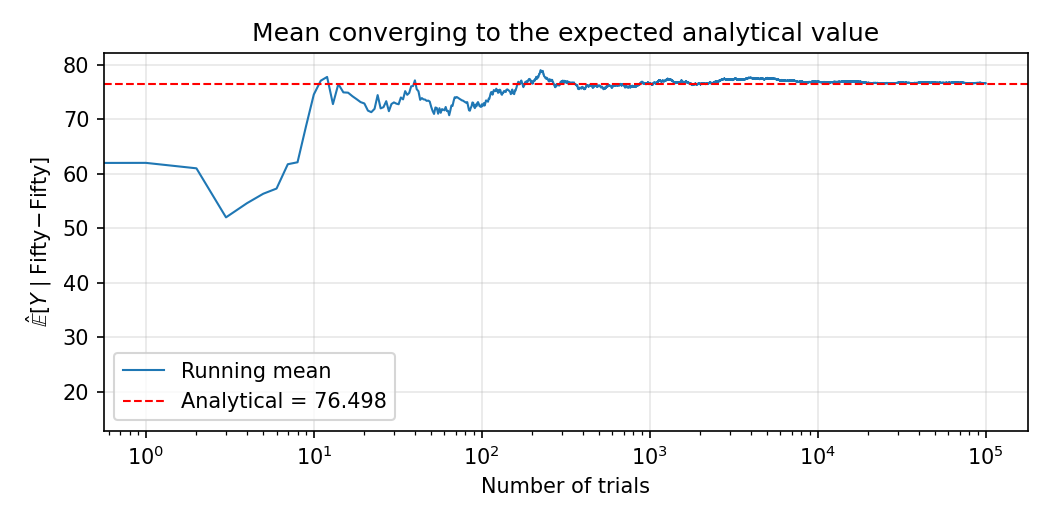
\includegraphics[width=0.6\textwidth]{outputs/fig_running_mean.png}
\caption{The running mean of $\hat{\mathbb{E}}[Y \mid \text{Fifty-Fifty}]$
converging as more trials are added. The horizontal axis is on log scale, and
the dashed line shows the analytical value.}
\end{figure}

\paragraph{Result.} Both simulated means (Fifty-Fifty and Guarantee) land inside the 95\%
confidence interval around the analytical value, which is a good indicator that the
simulator is correct and that we can trust our values.

\subsection{Q2: How does soft-pity onset change the full-kit distribution?}

Keeping everything else the same, we will try three different
character-banner soft-pity onsets: $n_s^c \in \{50, 60, 70\}$. Earlier
onset means the ramp starts sooner, so the 5-star probability hits
high values earlier in the pull sequence. For each onset we still simulate
$10^5$ trials.

\begin{table}[H]
\centering
\caption{Total pulls $T$ to complete the kit, by soft-pity onset.
$10^5$ trials each; 95\% CIs in brackets, computed using equation (4).}
\begin{tabular}{lrcrrr}
\hline
$n_s^c$ & Mean & 95\% CI & $Q_{0.50}$ & $Q_{0.90}$ & $Q_{0.99}$ \\
\hline
50 & $121.99$ & $[121.75,\,122.23]$ & $124$ & $179$ & $190$ \\
60 & $129.86$ & $[129.60,\,130.13]$ & $133$ & $195$ & $206$ \\
70 & $137.31$ & $[137.02,\,137.60]$ & $141$ & $211$ & $221$ \\
\hline
\end{tabular}
\end{table}

\begin{figure}[H]
\centering
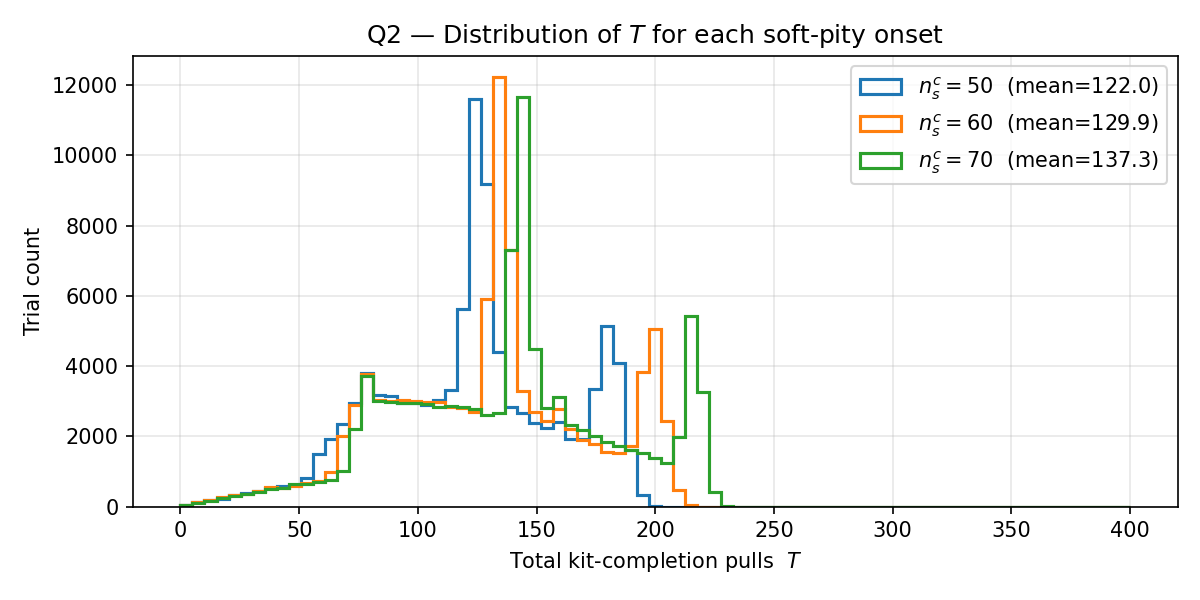
\includegraphics[width=0.65\textwidth]{outputs/fig_sensitivity.png}
\caption{Distribution of total full-kit pulls under each
soft-pity onset condition. Earlier onset shifts the whole distribution
left.}
\end{figure}

\paragraph{Result.} From what we find, the earlier the onset, the more the distribution
will shift left. It would also appear that the tail tends to shrink a little bit more than the mean. 
Moving $n_s^c$ from 70 to 50 drops the mean by about 15 pulls, or roughly
$11\%$. We also find that the 99th percentile drops significantly from 221 to 190 if we 
move the onset from 70 to 50. This is a large drop of about 14\%, which is 31 pulls. Considering that the tail
shrinks a bit faster than the mean, reducing the onset might be an effective way to help
balance the experience for unlucky players without affecting the average player too much. 

% =====================================================================
\section{Limitations and Future Work}
% =====================================================================

In our simulation, we use a linear ramp-up for the soft-pity system. Although this
simulation was supposed to simulate a gacha system, we should note that not all
gacha games use a linear soft-pity system. So the values and analysis we have found
may not necessarily be true in all real production gacha games. A future work
could analyze different soft-pity curves and see how that changes the pull distribution.

It should also be noted that most players will not start at exactly 0 initial pulls on a banner.
Players are actually able to save up pulls on one feature banner and the pity from the pull count
will transfer over to the next featured banner when the current one ends and the new one replaces it.
I mention this because this analysis paper does not entirely capture how the player would really approach
getting a featured character and their weapon in-game. There is actually some strategy involved
when planning to pull on a banner depending on what the player may want. A future work could
potentially numerically analyze an optimal strategy for a player to maximize how much they can get
out of a particular featured banner.

\end{document}
